\chapter{Clustering of CO emitters}

Galaxies are not distributed randomly in the universe. On the largest scales, the universe is isotropic and homogeneous, but on smaller scales, galaxies tend to cluster in space. One way to quantify how densely packed a population of galaxies is to compute the two-point correlation function. This allows for the measuring of the mass of the dark matter halos in which these galaxies reside \cite{hickox2011clustering}. For a certain redshift, the more clustered a population of galaxies is, the more massive the surrounding halo.

The clustering of different populations of galaxies has been constrained by previous works, some of which are summarized in Fig. \ref{fig:Hickox_compare}. The correlation length parameter, $r_0$, which is a proxy for the amplitude of the clustering, is shown in Fig. \ref{fig:Hickox_compare} as a function of redshift for different populations. \cite{10.1111/j.1365-2966.2011.20303.x} looks at the clustering in SMGs and compares their clustering to clustering found for other sets of astronomical objects, as can be seen in Fig. \ref{fig:Hickox_compare}. \cite{hickox2011clustering} found, in the Bo\"otes field, an $r_0$ for unobscured quasars to be $5.6 \pm 0.8$ at 0$<$z$<$1, and for obscured quasars $6.0 \pm 1.0 $. In \cite{10.1111/j.1365-2966.2011.20303.x}, submillimeter galaxies (SMGs) in the Extended Chandra Deep Field South were found to have a $r_0$ of $7.7_{-2.3}^{+1.8}$ at a 1$<$z$<$3. Other sources, such as \cite{adelberger2005spatial}, found for Lyman Break Galaxies (LBGs) $r_0$ values of $4.5 \pm 0.6$ at $z = 1.7$, $4.2 \pm 0.5$ at $z = 2.2$, and $4.0 \pm 0.6$ at $z = 2.9$, while \cite{ross2009clustering} found, for quasars in the Sloan Digital Sky Survey, an $r_0 = 5.45_{-0.45}^{+0.35}$ for z$\leq$2.2, both shown in Fig. \ref{fig:Hickox_compare}. The clustering of CO emitters has not been constrained as of yet because of the lack of large surveys targeting such objects. Wide ASPECS gives the possibility of providing some constraints on the clustering, and therefore putting constraints on the halo masses where these objects reside for the first time.

\begin{figure}[!htbp]
\centering 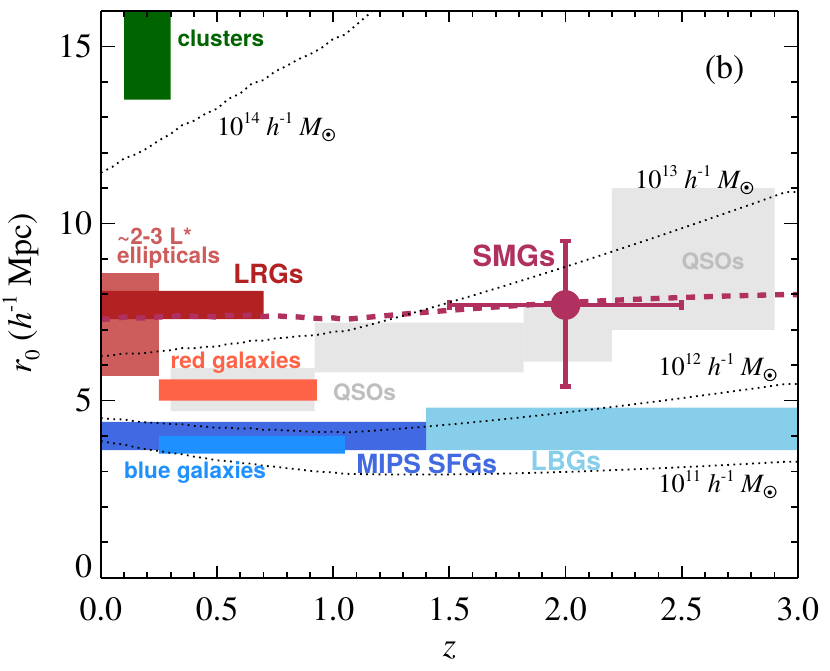
\includegraphics[width=87mm]{clustering/Hickox2012_Compare.png}
\caption{$r_0$ values for a variety of celestial objects as a function of redshift. The grey dotted lines show the evolution of $r_0$ for dark matter haloes of different masses. Figure adapted from \cite{10.1111/j.1365-2966.2011.20303.x}.}
\label{fig:Hickox_compare}
\end{figure}

\section{The Angular Correlation Function of CO Emitters}

The clustering is computed using a two-point correlation function. The two-point correlation function, $ \xi(r)$ is defined in terms of the probability $dP$ of finding a galaxy at a separation $r$ from another randomly chosen galaxy in a volume $dV$ above Poisson, such that \begin{equation}
    dP = n(1 + \xi(r))dV
\end{equation} where $n$ is the mean space density of the galaxies in the universe \cite{hickox2011clustering}, and $\xi(r)$ is normally modeled as a power-law such that $\xi(r)$ = $(\frac{r}{r_0})^{-\gamma}$. In practice, since the 3D separation $r$ between objects is hard to measure, the projected separations ($R$) or angular separations ($\theta$) are used instead. Here we focus in the computation of the angular auto-correlation function $\omega(\theta)$. This quantity can be computed using the estimator from \cite{1993ApJ...412...64L}, 
\begin{equation}
   \omega(\theta) = \frac{1}{RR}(DD-2DR + RR) 
\end{equation}\label{eq:Function} where $DD$, $DR$, and $RR$ are the number of data-data, data-random, and random-random galaxy pairs at a separation $\theta$. Each of the three collections is normalized to sum to one \cite{hickox2011clustering}. Here the 'data' catalog is represented by our actual CO emitter catalog of 35 sources with a fidelity $>$ 0.6, while the 'random' catalog is created by randomly distributing 20000 sources over the geometry of the survey, mimicking exactly the same area where CO emitters were detected. The distribution of data and random sources are shown in Fig. \ref{fig:Clustering_points}, and the angular correlation function, measured using Eq. 3.2, is shown in Fig. \ref{fig:Angular_binnings}.
%and the angular correlation function, measured using eq. XX is shown in Fig. XX

In order to check our code for the clustering computation, we created two additional random catalogs, of 20000 points each, and computed their angular correlation to show that it is consistent with zero, shown in Fig.\ref{fig:random_points}. The error bars for $\omega(\theta)$ are computed using Poisson errors for small statistics \cite{1986ApJ...303..336G}.

\begin{figure}[!htbp]
\centering 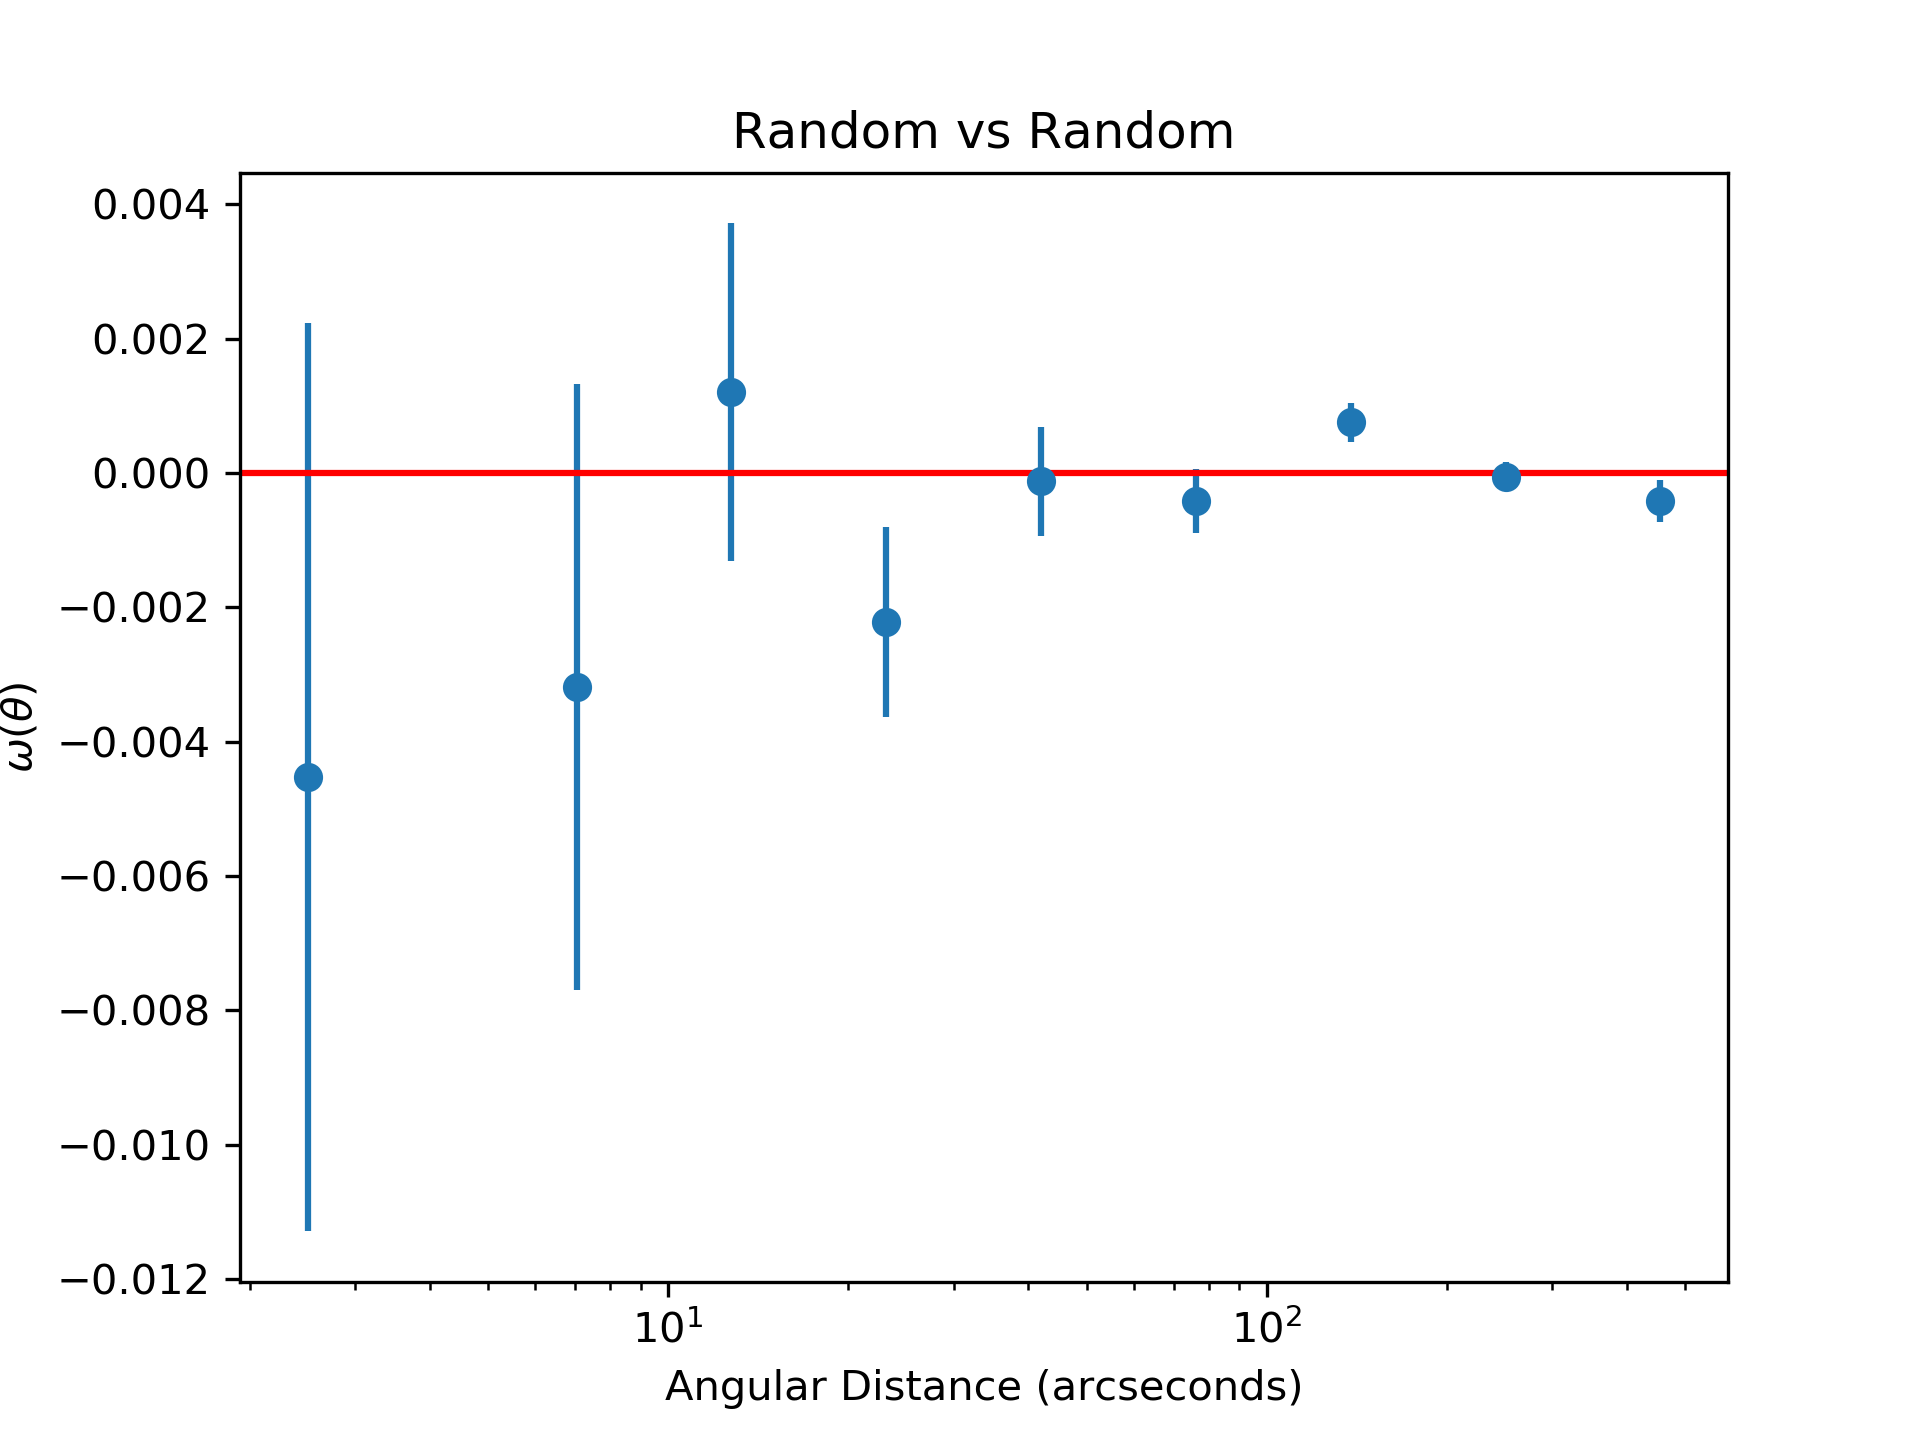
\includegraphics[width=100mm]{clustering/5Random_vs_Random_10000_bin9.png}
\caption{Angular correlation two sets of random points used in this analysis, showing that the angular correlation is consistent with zero, as would be expected for cross-correlating two sets of uniformly distributed points. The red line shows $\omega(\theta) = 0$.}
\label{fig:random_points}
\end{figure}

\begin{figure}[!htbp]
\centering 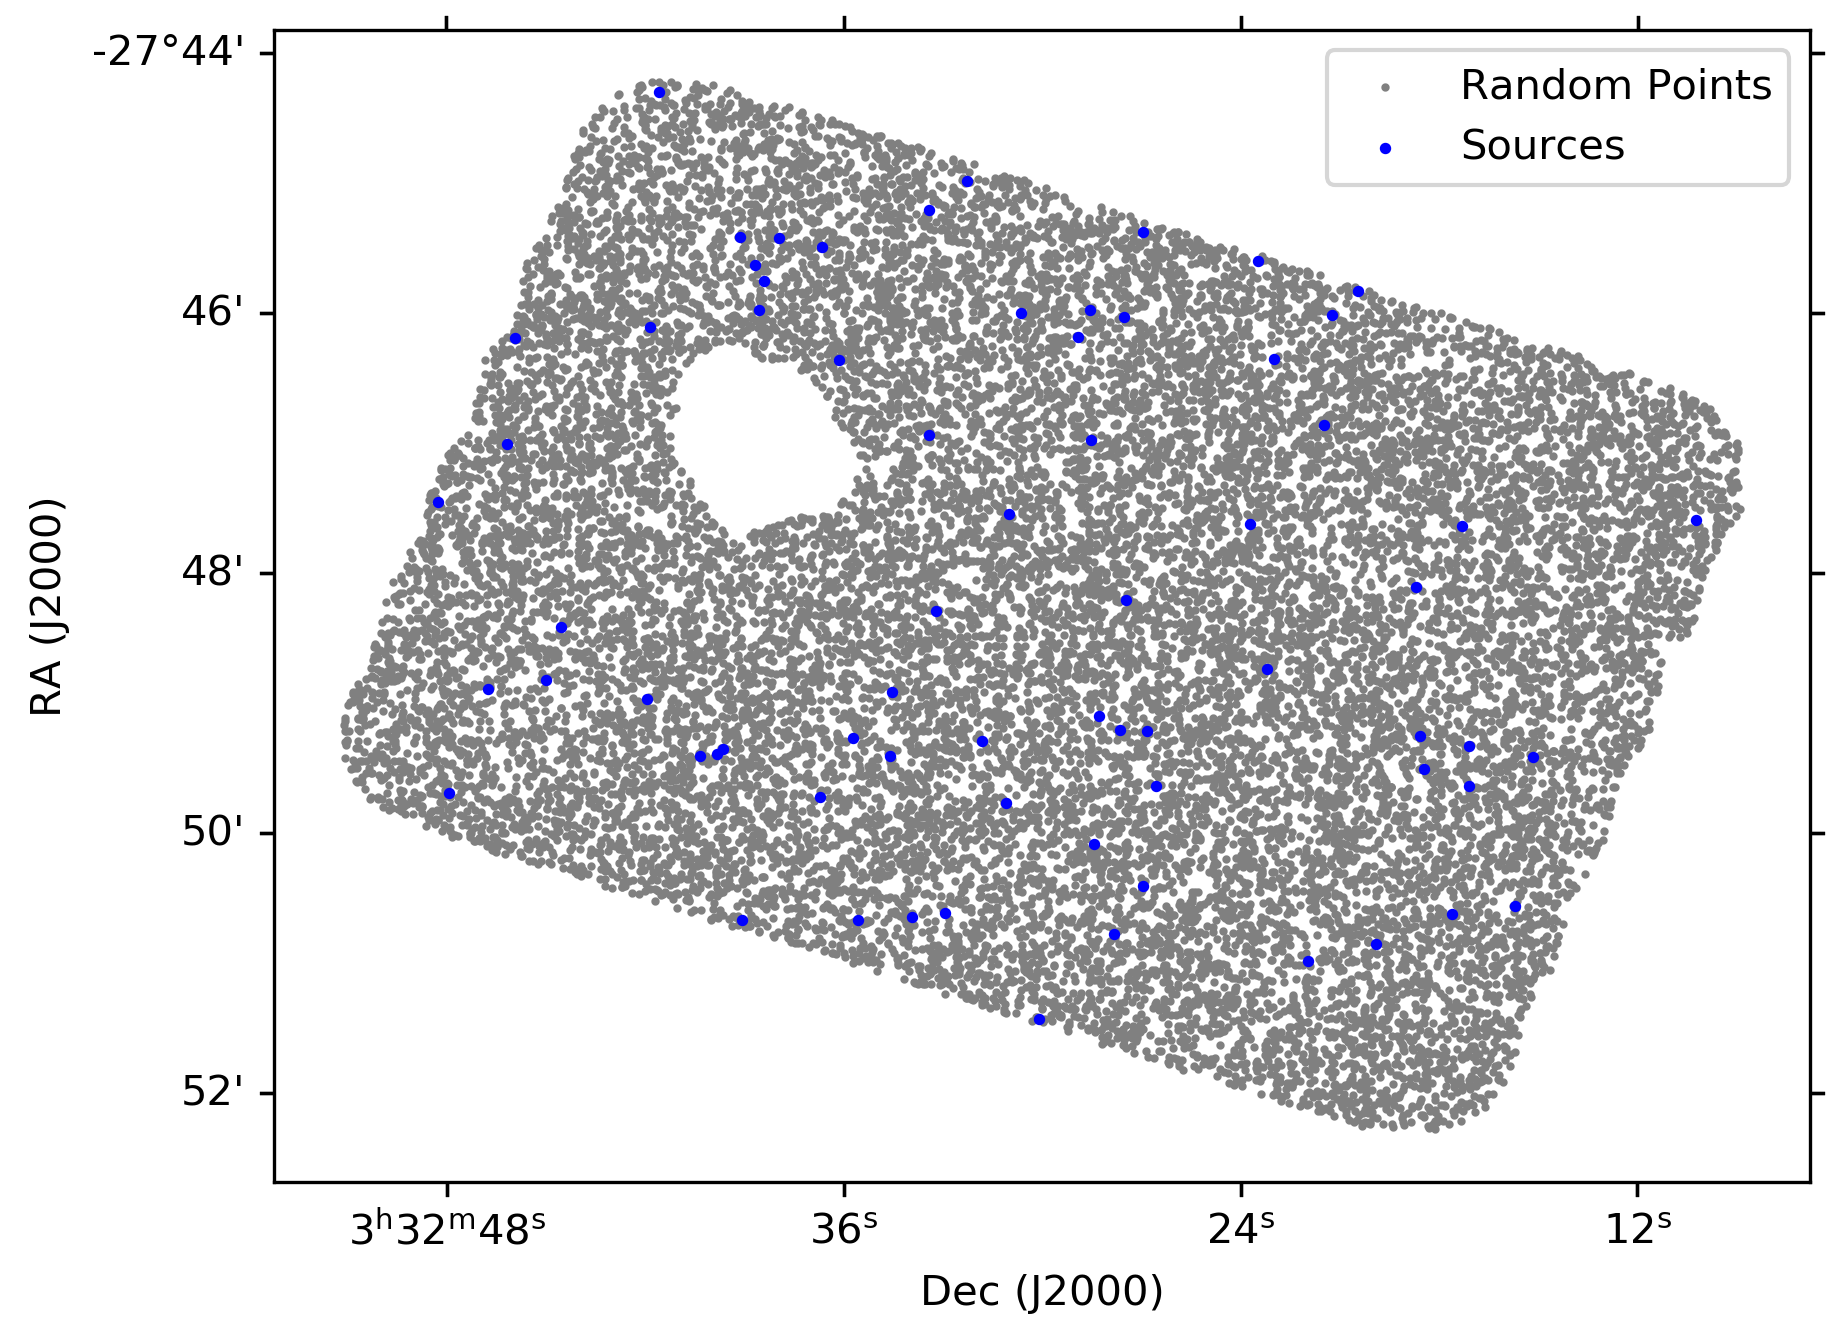
\includegraphics[width=120mm]{PDFS/NX_V_Y_Sources_20000.png}
\caption{Random points, in grey, and sources, in blue, from the $>$ 0.6 fidelity cut. The random points are distributed uniformly throughout the Wide ASPECS footprint.}
\label{fig:Clustering_points}
\end{figure}

Once the angular correlation function is found, a power-law model is fitted following 
\begin{equation}
    \omega(\theta) = A\theta^{-\beta} 
\end{equation} where $\beta$ = 0.8, as used for many other galaxy angular correlations \cite{hickox2011clustering}. The data is fitted twice, once for all the binned data, and once fitting only to the bins with positive values. Because of the small size of the sample, our measurement is noisy and at some scales the observed correlation function becomes negative. These negative values are most likely the result of statistical fluctuations. 

\subsection{Obtaining $r_0$ and $\gamma$}

Two equations are used to convert the $A$ and $\beta$ to real-space $r_0$ and $\gamma$, 

\begin{equation}
    \gamma = \beta + 1
\end{equation} and \begin{equation}
    A = H_{\gamma}\frac{\int_{0}^{\inf} (dN_1/dz)(dN_2/dz)E_z\chi^{1 - \gamma} dz}{[\int_{0}^{\inf} (dN_1/dz)dz][\int_{0}^{\inf} (dN_2/dz)dz]}r_0^{\gamma}
\end{equation}

where $H_{\gamma} = \Gamma(0.5)\Gamma(0.5[\gamma -1])\Gamma(0.5\gamma)$, with $\Gamma$ being the gamma function, and $\chi$ the radial comoving distance. $dN_{1,2}/dz$ are the redshift distributions of the samples, where in the case of autocorrelation are equal to each other, and $E_z = H_z/c = dz/d\chi$ \cite{hickox2011clustering}. The Hubble parameter $H_z$ can be found from
\begin{equation}
    H_z^2 = H_0^2[\Omega_m(1+z)^3 + \Omega_{\lambda}]
\end{equation}\cite{hickox2011clustering}.

For this analysis, the redshift distribution was taken from the CO redshifts of the lines and the calculations were performed over the range z = 1.5 to 3.5, as this is the range where most of the CO candidates seem to lie. To calculate $dN_{1,2}/dz$, the redshift distribution of the CO lines was fitted with a Gaussian, and the integral was taken over the Gaussian fit. The angular correlation function was computed over the range of 8.39 to 582.10 arcseconds, using logarithmically spaced bins. Because there are only 35 line candidates in the catalog, the clustering measurements are quite noisy. The final calculated values are $r_0 = 6.96_{-0.82}^{+0.75}$, and $\gamma = 1.8$ when using the values of all the bins for fitting. This result is consistent within the error bars with the $r_0$ value obtained when only positive values are fitted as shown in Fig. \ref{fig:Angular_binnings}. Table \ref{table:Angular_binnings} shows the bin values and errors displayed in Fig. \ref{fig:Angular_binnings}.

\begin{figure}[!htp]
\centering 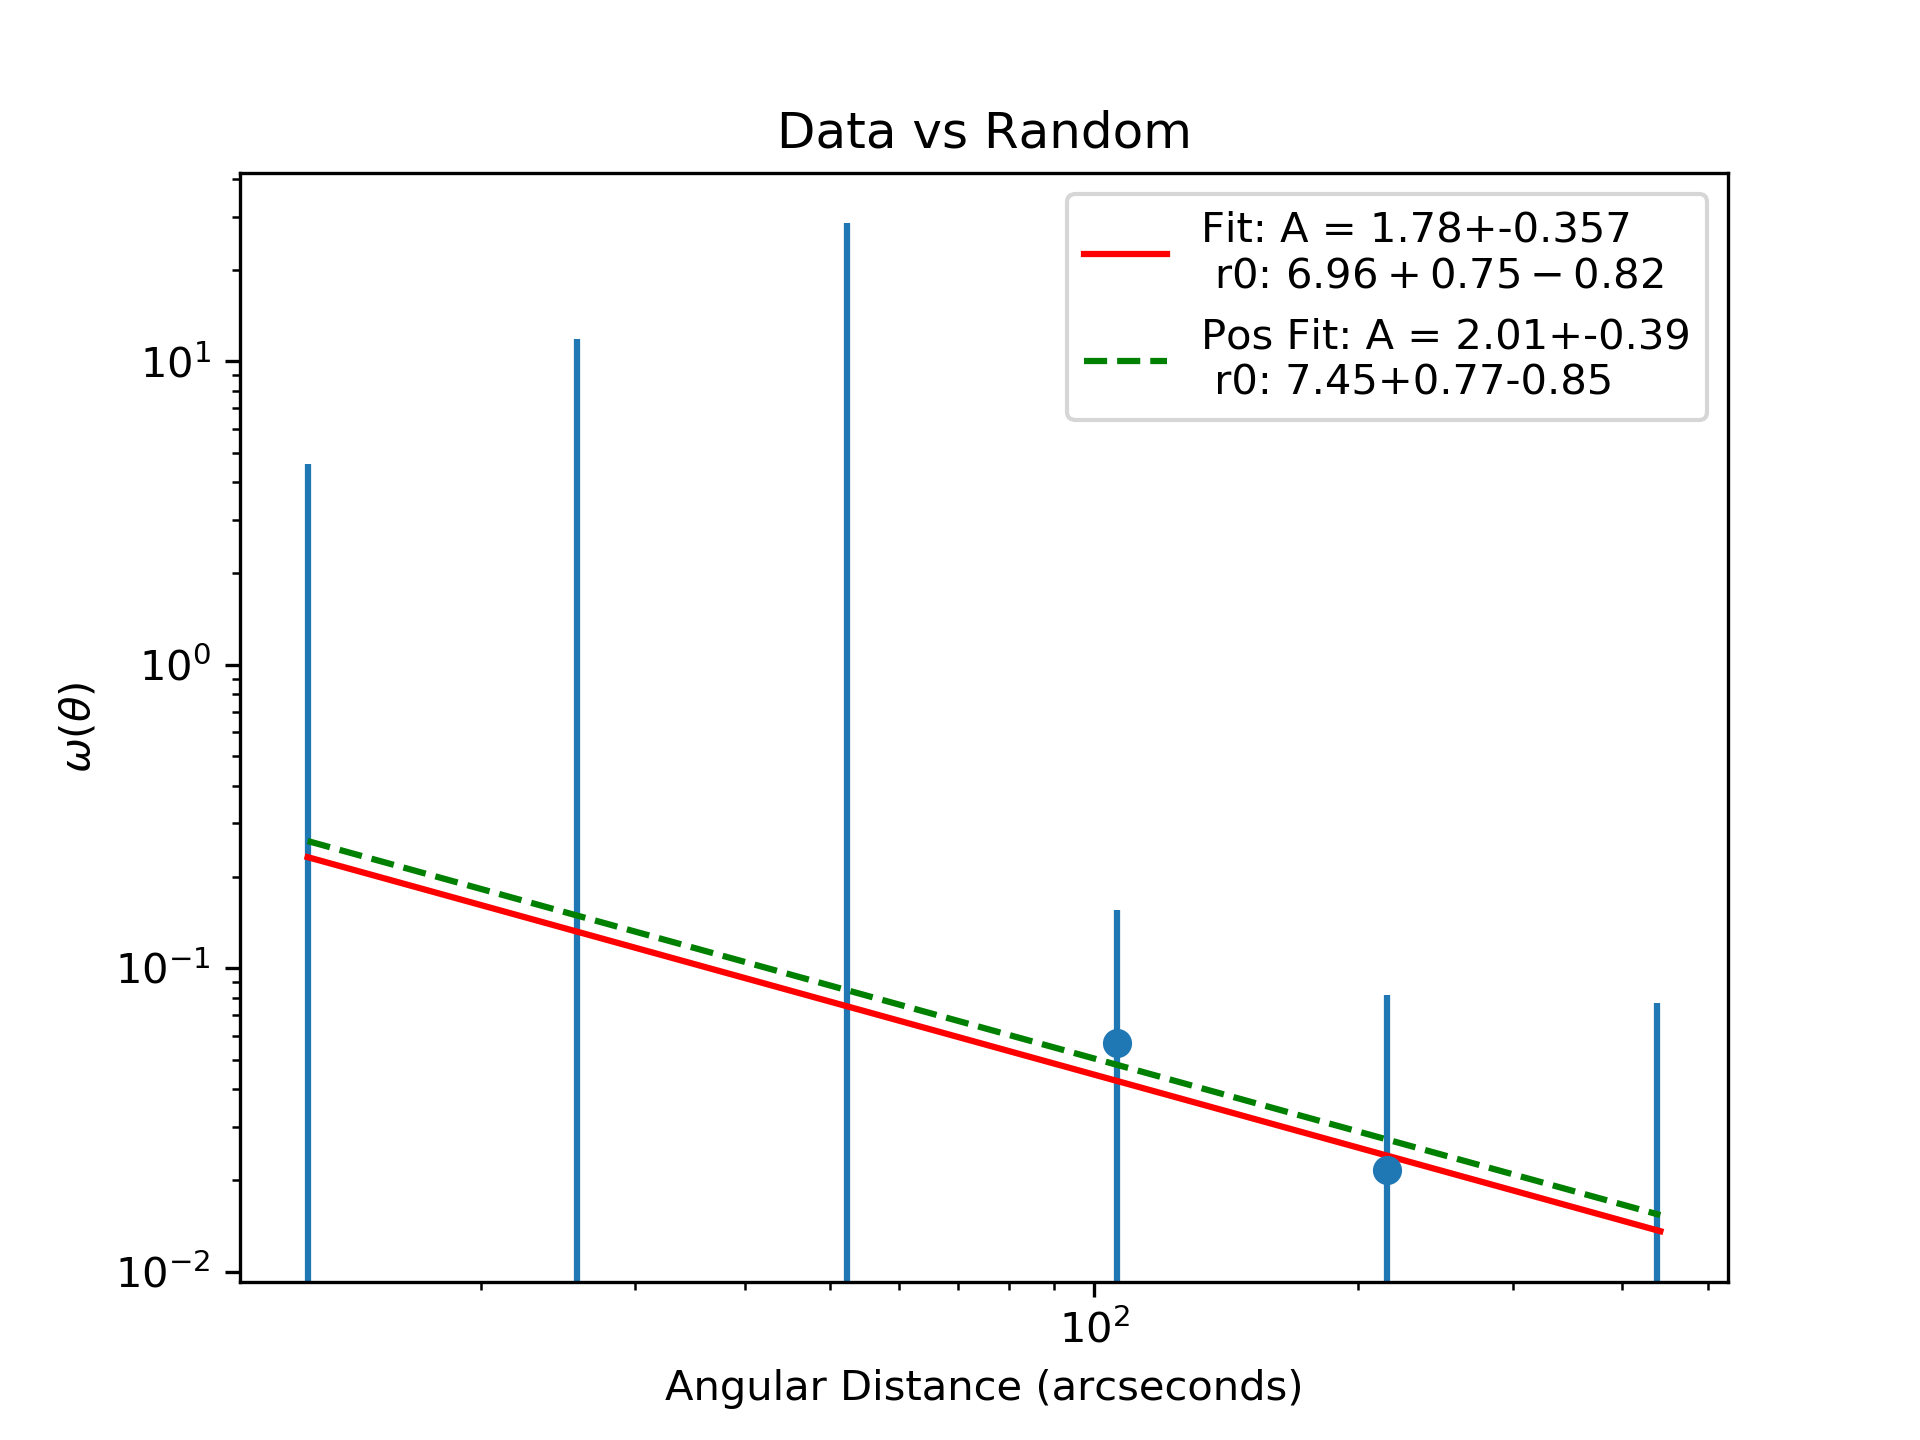
\includegraphics[width=90mm]{clustering_two/Data_vs_Random_20000_bin6_sn0_6_NFalse.png}
\caption{Angular correlation function for 6 bins for the chosen fidelity cut of 0.6. Red is the fit $\omega(\theta) = A\theta^{-0.8}$ to all the bins, while the green line is the fit to only bins with positive values. This is the final binning used for the analysis. }
\label{fig:Angular_binnings}
\end{figure}

\begin{table}[!htp]
\caption{$\omega(\theta)$ values for a given $\theta$ for the fidelity $>$ 0.6 catalog. The $\theta$ given is the center of each bin. Errors are calculated using Poisson errors for small statistics \cite{1986ApJ...303..336G}.}
\centering
\begin{tabular}{cc}\label{table:Angular_binnings}
$\theta$ & $\omega(\theta)$          \\
\hline
12.70    & $-0.04_{-0.71}^{+4.64}$   \\
25.79    & $-0.06_{-5.232}^{+11.95}$ \\
52.33    & $-0.31_{-18.24}^{+28.87}$ \\
106.21   & $0.06_{-0.10}^{+0.10}$    \\
215.54   & $0.02_{-0.06}^{+0.06}$    \\
437.42   & $0.00_{-0.08}^{+0.08}$   
\end{tabular}
\end{table}

\section{Discussion}\label{sec:Clust_Disc}

In comparison to previous results, the $r_0$ of the CO emitters here are quite similar to the values for the SMGs found in \cite{10.1111/j.1365-2966.2011.20303.x} for a similar redshift range, and quasars in the Bo\"otes field at a lower redshift \cite{hickox2011clustering}, while being slightly more clustered than the quasars found in \cite{ross2009clustering}. In comparison to other populations of celestial objects shown in Fig. \ref{fig:Hickox_ASPECS}, the clustering for CO emitters seems to be significantly stronger than for the Lyman Break Galaxies in \cite{adelberger2005spatial}, which covers the same redshift range of 1.5$<$z$<$3.5. Based on the models shown in Fig. \ref{fig:Hickox_ASPECS}, our results implies that the dark matter halos surrounding these CO emitters would be in the range very roughly between $10^{12} h^{-1}M_{\odot}$ and $10^{13} h^{-1}M_{\odot}$.

\begin{figure}[!htbp]
\centering 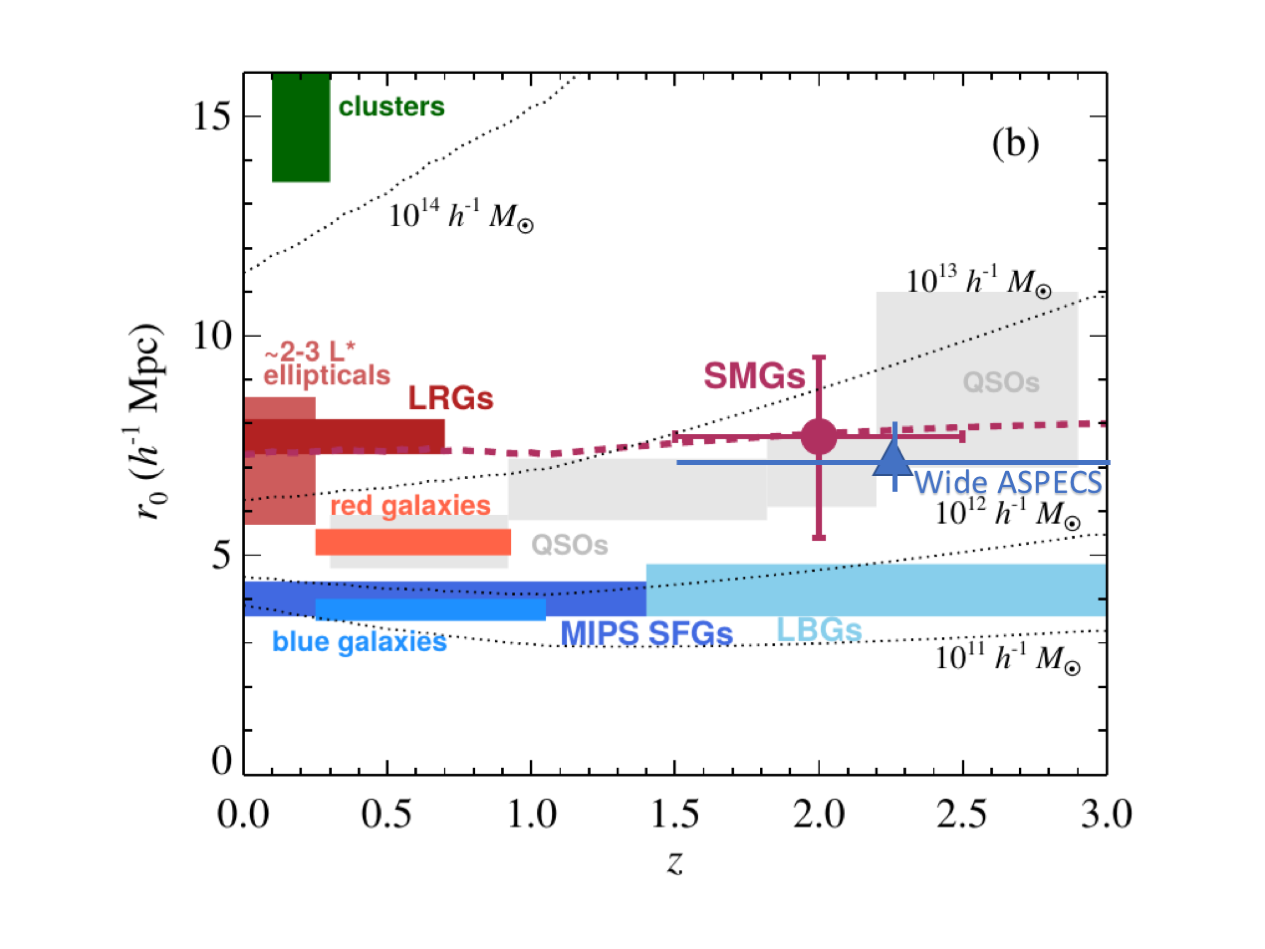
\includegraphics[width=120mm]{clustering/Hickox_WideASPECS.png}
\caption{$r_0$ as derived from Wide ASPECS CO emitters with a fidelity $>$ 0.6, in comparison to other types of celestial objects as a function of redshift. Wide ASPECS is the blue triangle, with the error bars being the error on $r_0$ in y, and the redshift range covered in x, extending from z=1.5 to z=3.5. The grey dotted lines show the evolution of $r_0$ for dark matter haloes of different masses. Figure adapted from \cite{10.1111/j.1365-2966.2011.20303.x}.}
\label{fig:Hickox_ASPECS}
\end{figure}

As an interesting test, the two-point correlation function was also computed for other fidelity cuts. As can be seen in Fig. \ref{fig:Angular_correlation}, as the fidelity increases (i.e. the sample is more restricted to contain more real sources and less contamination by noise), $A$ increases as well. When converted to $r_0$, the fidelity cuts result in $r_0$ values of $7.8_{-7.8}^{+5.78}$ for fidelity $>$ 0.7, $6.96_{-0.82}^{+0.74}$ for fidelity $>$ 0.6, $0.0_{-0.0}^{+4.32}$ for fidelity $>$ 0.5, and $r_0 = 0.0_{-0.0}^{+3.83}$ for fidelity $>$ 0.4. This increasing $r_0$ as the fidelity increases is the expected behavior, since for low fidelity cuts, we are including more false detections (noise) that are probably randomly distributed over the area of Wide ASPECS, and so the  clustering signal of the real detections is diluted.  As we cut at higher fidelities, the signal is less diluted by the contamination of this noise, and so we are able to measure a more realistic clustering. We recall however that our measurements are still noisy and improvements need to be done to increase the signal to noise of this measurement.  

\begin{figure}[!htbp]
\centering 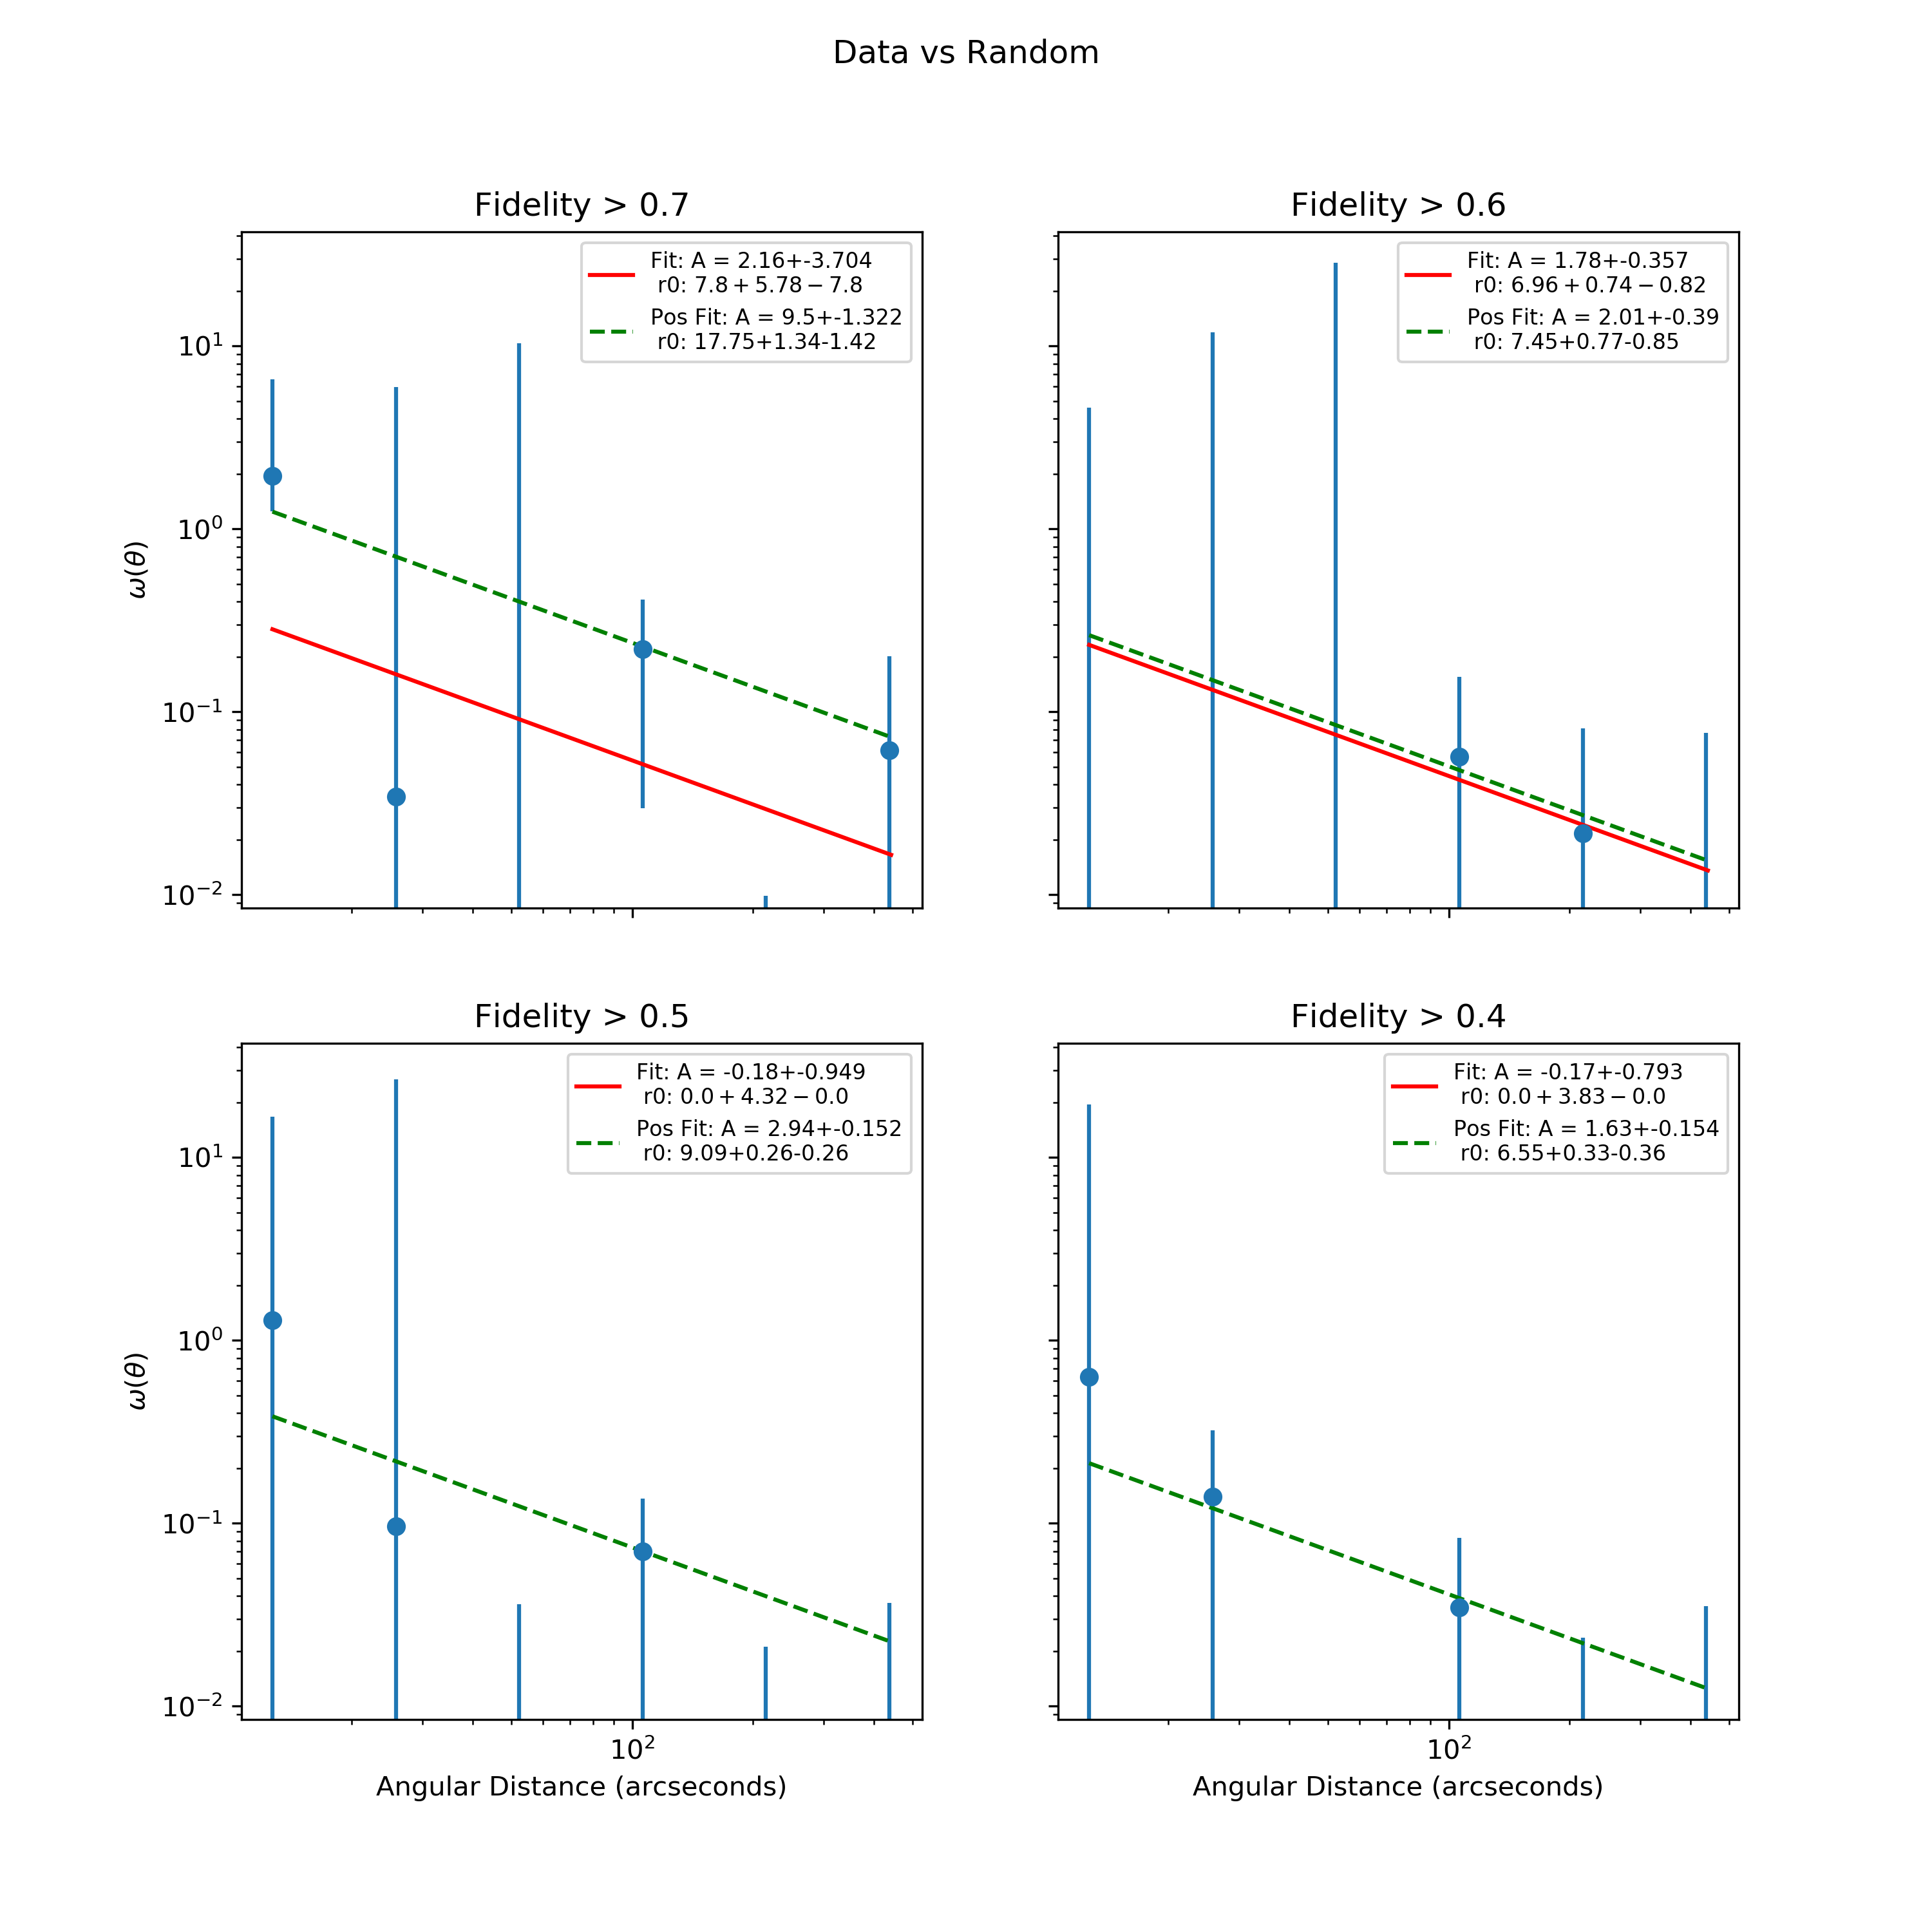
\includegraphics[width=160mm]{FINAL_Log_4Panel_Data_Vs_Random_bin6_NFalse_Num20000.png}
\caption{Angular correlation function for various fidelity cuts. The bins increase logarithmically from 8.39 arcsecs to 582.10 arcseconds. The red lines are from fitting $\omega(\theta) = A\theta^{-0.8} $ to all of the bins. The green dashed line is from fitting that same equation only to bins that had a positive value. The yellow dashed line is the fit from the fidelity $>$ 0.4 catalog. As the fidelity goes up, the $A$ value increases as well, indicating stronger clustering. The few line candidates mean that the results are quite noisy, and are sensitive to the bins chosen.}
\label{fig:Angular_correlation}
\end{figure}

% Do something with the dependent on the binning
Besides the different fidelity cuts, different distance binnings also are included to study their effects on the final $r_0$ results. The results seem to be dependent on the binning. While the values for the only positively-fitted bins does not change dramatically as the binning changes, the number of bins does make a large difference in the final $A$, and therefore $r_0$ values, shown in Figures \ref{fig:Angular_bin_8} and \ref{fig:Angular_bin_5} in comparison to Fig. \ref{fig:Angular_binnings}. The range in the $r_0$ values underlines how the low statistics available makes the clustering measurement very noisy, even though all the $r_0$ values for the fidelity $>$ 0.6 sample are consistent with each other. Although the measurement of the angular correlation function gives us a preliminary result about the clustering of these sources, the small size of our sample does not allow us to accurately determine the clustering only based on the auto-correlation technique, and other more sophisticated methods need to be employed to improve the statistics of the measurement. This is further discussed in section \ref{sec:Future_Work}.

\begin{figure}[!htbp]
\centering 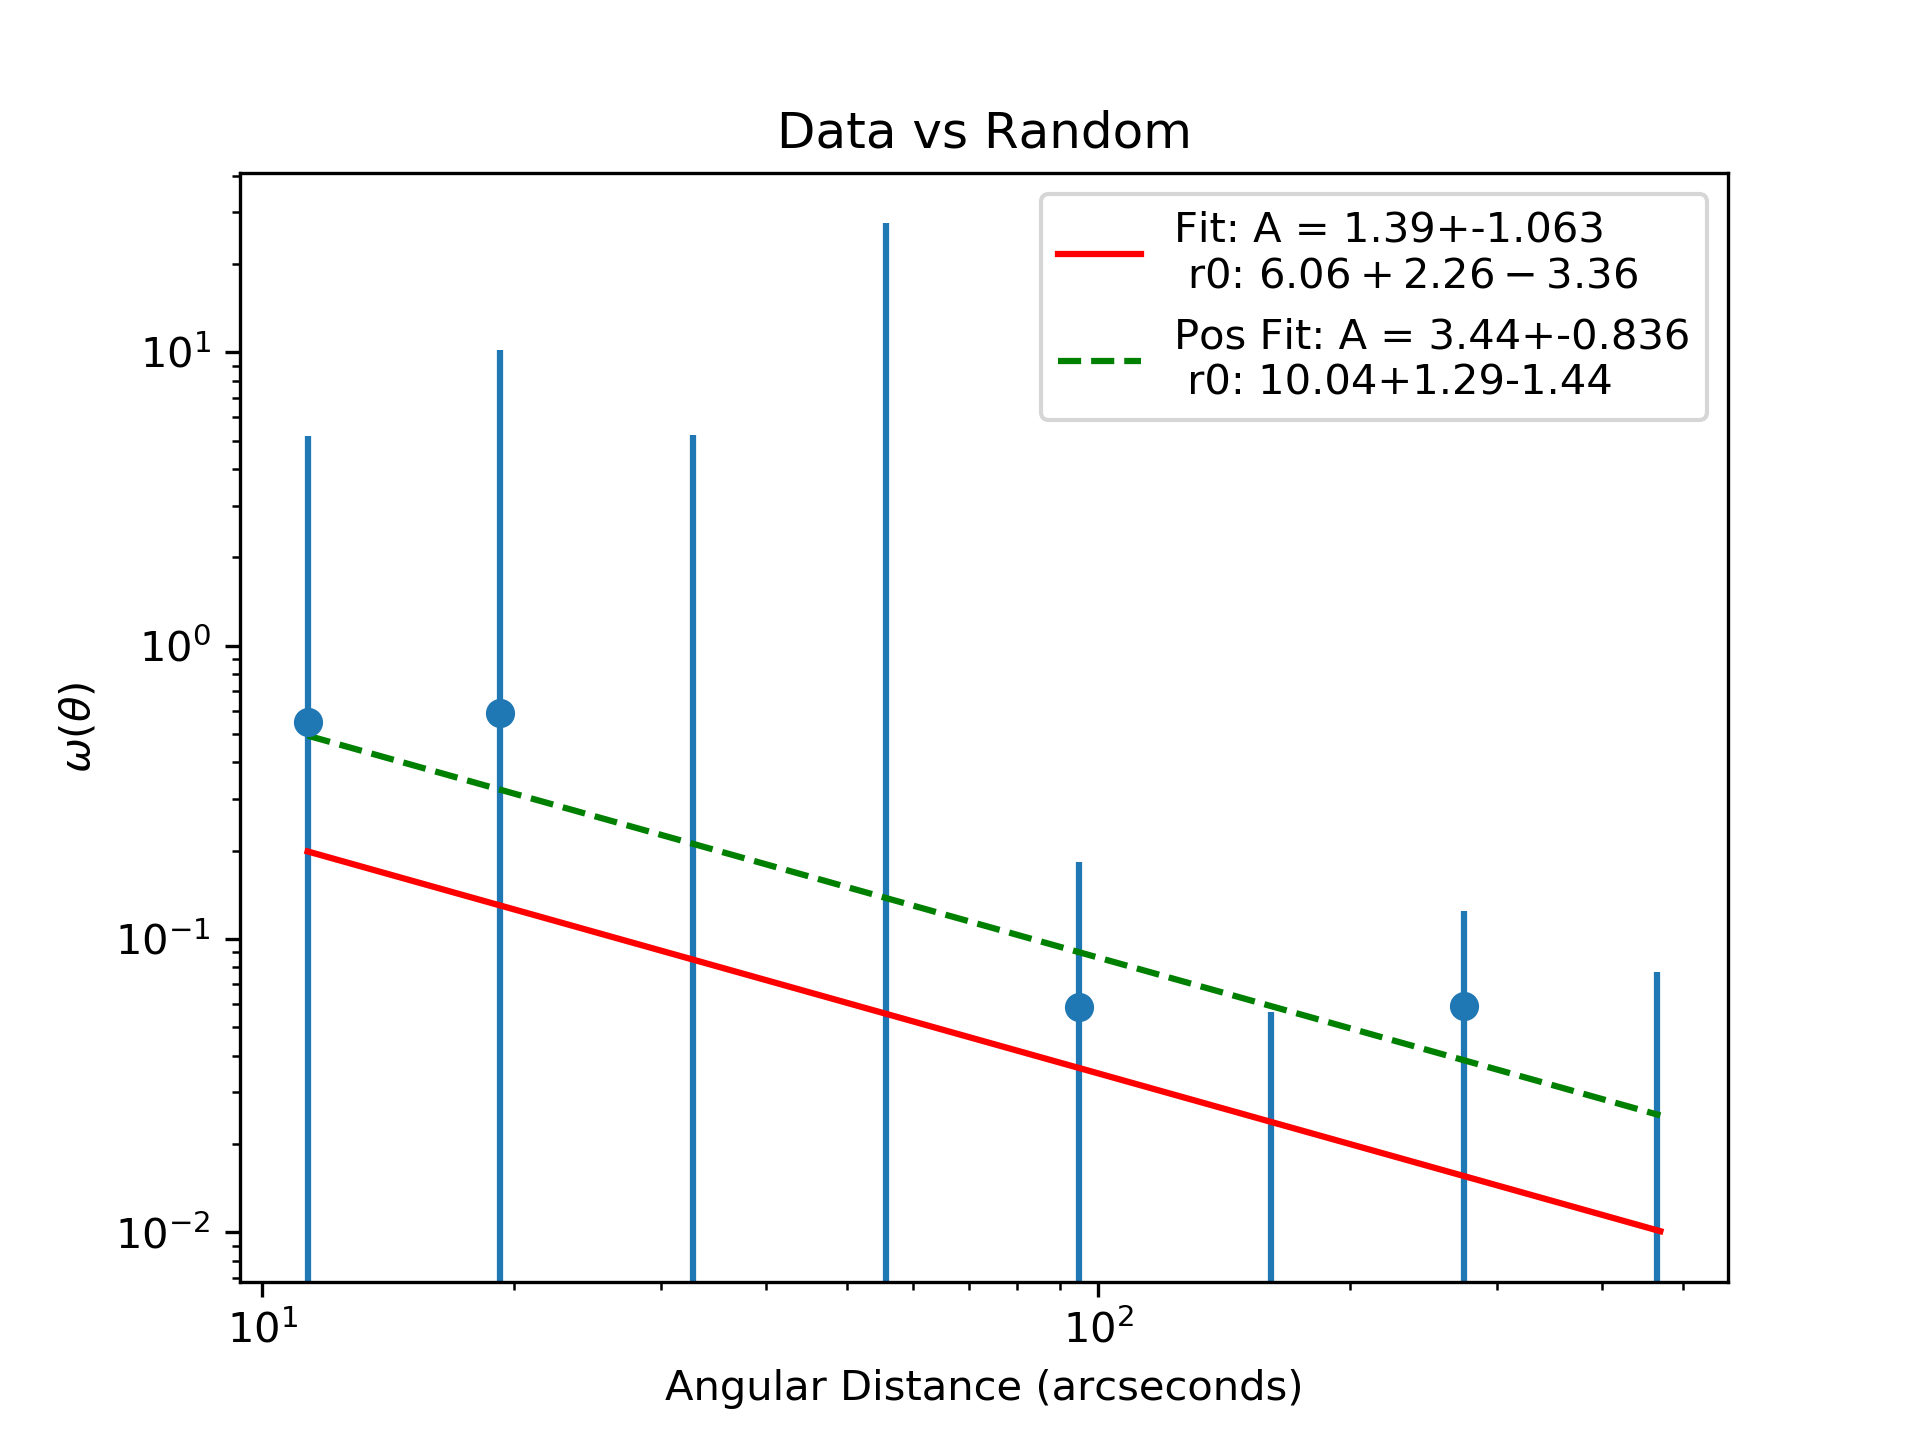
\includegraphics[width=90mm]{clustering_two/Data_vs_Random_20000_bin8_sn0_6_NFalse.png}
\caption{Angular correlation function for 8 bins  for fidelity $>$ 0.6. In this case, an increase in the number of bins decreases the $r_0$ value, although it is still consistent with the original $r_0$ value from \ref{fig:Angular_binnings}.}
\label{fig:Angular_bin_8}
\end{figure}

\begin{figure}[!htbp]
\centering 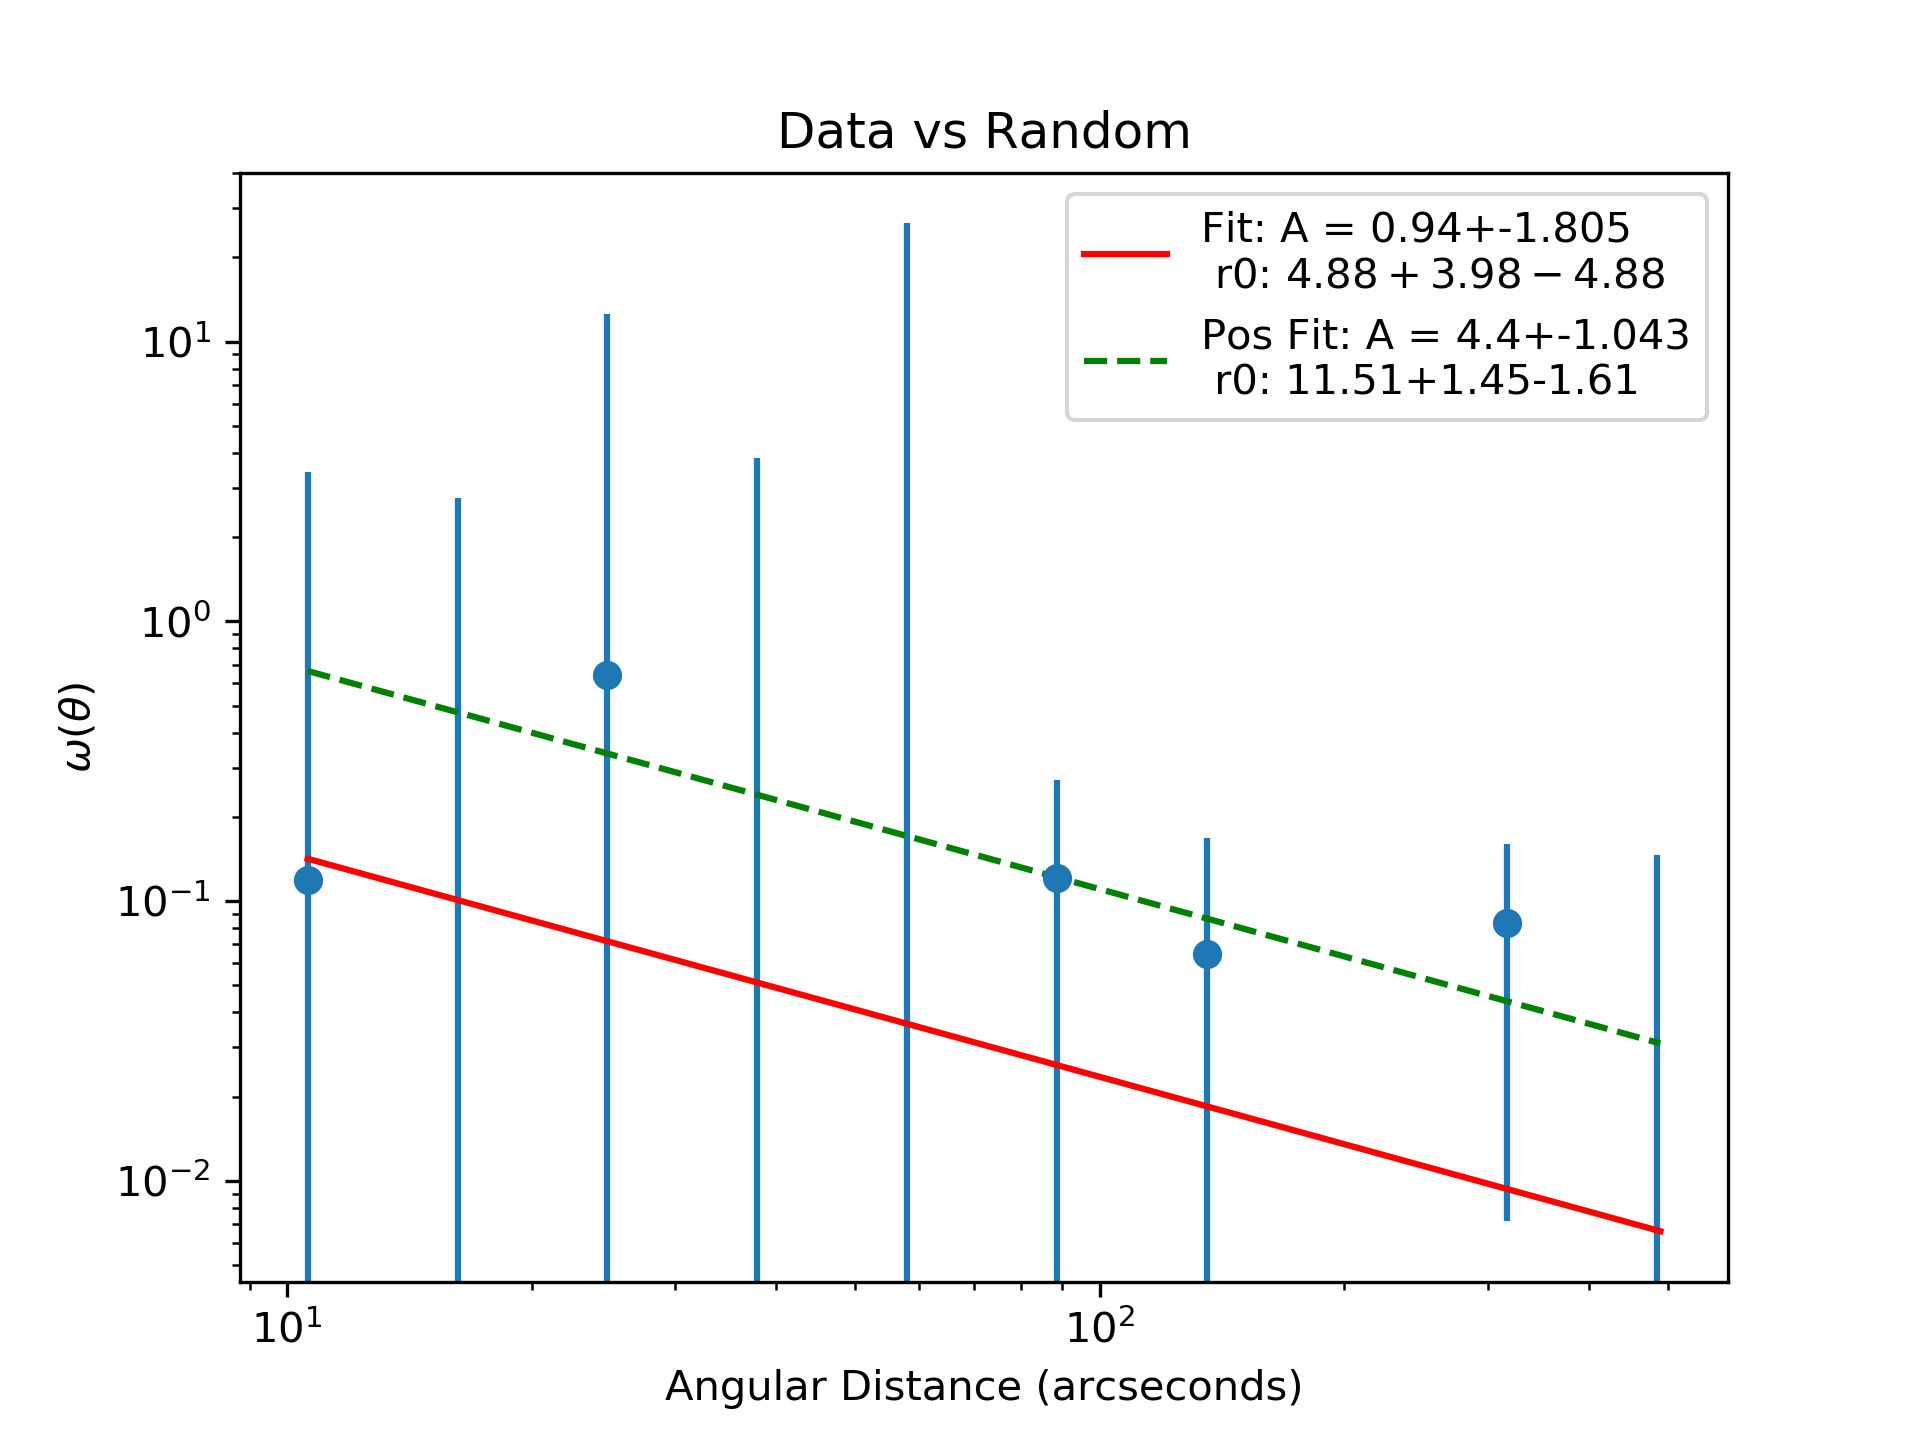
\includegraphics[width=90mm]{FINAL_Data_vs_Random_20000_bin10_sn0_6_NFalse.png}
\caption{Angular correlation function for 10 bins for fidelity $>$ 0.6. In this case, further increasing the number of bins also decreases the $r_0$ value, which is still consistent with the $r_0$ found in \ref{fig:Angular_binnings}. This could be a result of the very low statistics and so extremely noisy measurements.}
\label{fig:Angular_bin_5}
\end{figure}

The existence of negative values in the correlation function means that there are fewer numbers of data-data pairs in that bin compared with expectation, which could happen when a field is underdense. However, in that case, we would expect that all the points would be systematically negative. So in this case it is most likely related with the extremely high noise in the measurement. This could partially explain why, as the number of bins is increased, $r_0$ continues to decrease. 

% Random points: 582.10 arcseconds, DD points, 516 arcseconds

